\documentclass[tikz]{standalone}
\usepackage{pgfplots}
\pgfplotsset{compat=1.15}
\usepackage{mathrsfs}
\usetikzlibrary{arrows,calc}
\usepackage{tkz-euclide}
\pagestyle{empty}

\definecolor{AngleClr}{rgb}{0,0.39215686274509803,0}
\definecolor{ShapeClr}{rgb}{0.6,0.2,0}

\definecolor{BlueClr}{RGB}{71, 113, 158}
\definecolor{GreenClr}{RGB}{129, 196, 120}
\definecolor{RedClr}{RGB}{204, 98, 59}

\begin{document}

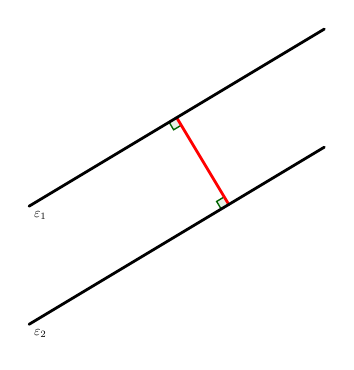
\begin{tikzpicture}[scale=.75]
\tkzSetUpLine[line width=1pt,color=black]
\tkzSetUpPoint[fill=black]

\tkzDefPoints{0/0/A,5/3/B,0/-2/C,5/1/D,2.5/1.5/E}


\tkzDefPointBy[projection=onto C--D](E)\tkzGetPoint{F}

\tkzMarkRightAngles[line width=0.5pt, size=.15,color=AngleClr,fill=AngleClr,fill opacity=0.1](F,E,A E,F,C)

% \tkzDrawSegments[line width=0.5pt,color=black,dashed,dash pattern=on 1pt off 1.75pt](B,H B1,H C,C1 A,B2 B2,B1 C2,A2)
% \tkzDrawSegments[line width=0.5pt,color=black,dashed,dash pattern=on 1pt off 1.75pt,add=0 and 0.3](A,H)
\tkzDrawSegments[line width=1pt,color=red](E,F)
\tkzDrawSegments[line width=1pt,color=black](A,B C,D)

\tkzLabelPoint[below right,scale=0.5](A){$\varepsilon_1$}
\tkzLabelPoint[below right,scale=0.5](C){$\varepsilon_2$}

% \tkzMarkSegments[mark=s||,size=2.5](O,A O,B O,C)

\end{tikzpicture}

\end{document}
